\documentclass[12pt,a4paper]{article}
\usepackage[utf8]{inputenc}
\usepackage{graphicx}
\usepackage{color}
\usepackage[magyar]{babel}
\usepackage{listings}
\usepackage{float}

\usepackage{enumerate}
\usepackage{tikz}
\usetikzlibrary{shapes,arrows}
\usetikzlibrary{positioning}
\usetikzlibrary{arrows.meta}

\tikzset{
block/.style = {draw, fill=white, rectangle, minimum height=3em, minimum width=3em},
tmp/.style  = {coordinate}, 
input/.style = {coordinate},
output/.style= {coordinate},
pinstyle/.style = {pin edge={to-,thin,black}
}
}
\usepackage[siunitx]{circuitikz} 
\renewcommand{\lstlistingname}{Lista}
\usepackage{hyperref}
\hypersetup{
	pdftitle={HA5KFU tanfolyam - Modulációs workshop},
	pdfauthor={HA5KFU Rádióamatőr Klub},
	pdfsubject={HA5KFU tanfolyam},
	pdfcreator={latex},
	pdfkeywords={ },
	pdfpagemode=UseOutlines,
	pdfdisplaydoctitle=true,
	pdflang=hu,
	unicode
}
\usepackage{color} %red, green, blue, yellow, cyan, magenta, black, white
\definecolor{mygreen}{RGB}{28,172,0} % color values Red, Green, Blue
\definecolor{mylilas}{RGB}{170,55,241}
\lstset{language=Matlab,%
	basicstyle=\scriptsize\ttfamily,
    %basicstyle=\color{red},
    breaklines=true,%
    morekeywords={matlab2tikz},
    keywordstyle=\color{blue},%
    morekeywords=[2]{1}, keywordstyle=[2]{\color{black}},
    identifierstyle=\color{black},%
    stringstyle=\color{mylilas},
    commentstyle=\color{mygreen},%
    showstringspaces=false,%without this there will be a symbol in the places where there is a space
    numbers=left,%
    numberstyle={\tiny \color{black}},% size of the numbers
    numbersep=9pt, % this defines how far the numbers are from the text
    emph=[1]{for,end,break},emphstyle=[1]\color{red}, %some words to emphasise
    %emph=[2]{word1,word2}, emphstyle=[2]{style},    
}

\pagestyle{plain}
\sloppy
\begin{document}
\begin{center}

\includegraphics[width=300pt,keepaspectratio]{figures/ha5kfu.eps}
\\[0.5cm]
Rádióamatőr tanfolyamot segítő jegyzet, egyelőre kidolgozás alatt \\
Összeállította: Bazsó Márton, Szabó Áron % Feel free to add yourself
\\[1cm]

{\huge \bfseries Modulációs workshop \\[2cm]}



\end{center}

\renewcommand{\contentsname}{Tartalom}\tableofcontents 
\newpage

\newpage

\section{Bevezető}
A workshop célja bemutatni a különböző modulációs eljárások idő- és frekvenciatartománybeli viselkedését, illetve matematikai leírásukat. 

\section{Előkészületek}
A workshop Octave-ban és Matlab-ban is elvégezhető, a használt parancsok mindkettőben működőképesek.

\paragraph{Octave telepítés:} 
\begin{itemize}
	\item \textbf{GNU Octave telepítése:} \\\url{https://wiki.octave.org/Category:Installation}
	\item \textbf{Signal package telepítése:} Octave-on belül: 	\\
	\texttt{pkg install -forge signal}\\
	Ha ez valamiért nem működne, akkor Ubuntun command line-ból is telepítheted: \texttt{sudo apt-get install octave-signal}
\end{itemize}

\section{Feladatok}

\subsection{Szinusz jel generálása, ábrázolása}
Első feladatunk egy szinusz jel generálása lesz, melyet a \textit{sin()} függvénnyel tehetünk meg. Fontos, hogy ez a függvény egy adott érték szinuszát adja vissza, nekünk viszont egy időtartománybeli függvényre van szükségünk. 

Létre kell hoznunk tehát egy időtengelyt, aminek pontjaiban kiszámoljuk a függény értékét. Ebből a szempontból fontos meghatározni a mintavételi frekvenciát ($F_s$), hiszen ebből az értékből számolható, hogy két minta közt mennyi idő fog eltelni. Válasszuk a mintavételi frekvenciát \textit{44 100 Hz}-re, ami a digitális audió jelfeldolgozásban használatos frekvencia, és a számítógép hangkártyáján könnyen lejátszható.

Ha a minták számát ($N$) másodpercben szeretnénk megadni, egyszerűen szorozzuk meg a másodperc értéket a mintavételi frekvenciával. A másodperc időtengelyt ($t$) úgy kaphatjuk meg, ha az \texttt{1:N} sorozatot elemenként elosztjuk a mintavételi frekvenciával (a transzponálásra azért van szükség, hogy oszlopvektort kapjunk). Ez után a szinusz jel egyszerűen kiszámolható: mivel a szinusz egy periódusa $2\pi$, a szinuszjel pillanatnyi értékét $t \cdot f \cdot 2\pi$-re kell választani, ahol $f$ a szinusz frekvenciája.

\begin{lstlisting}[frame=single,language=matlab,caption=Mintavételi frekvencia beállítása és szinuszjel előállítása]
Fs = 44100; % mintaveteli freki
l = 1.5; % minta hossza masodpercben
N = l * Fs, % mintak szama
f = 440; % 20 Hz-es lesz a jel
t = ( 1:N )' ./ Fs; % Ido oszlopvektora
y = sin( t * f * 2 * pi );
plot( t, y );
\end{lstlisting}

Ábrázoljuk a Plot függvénnyel időtartományban:

\begin{figure}[H]
\begin{center}
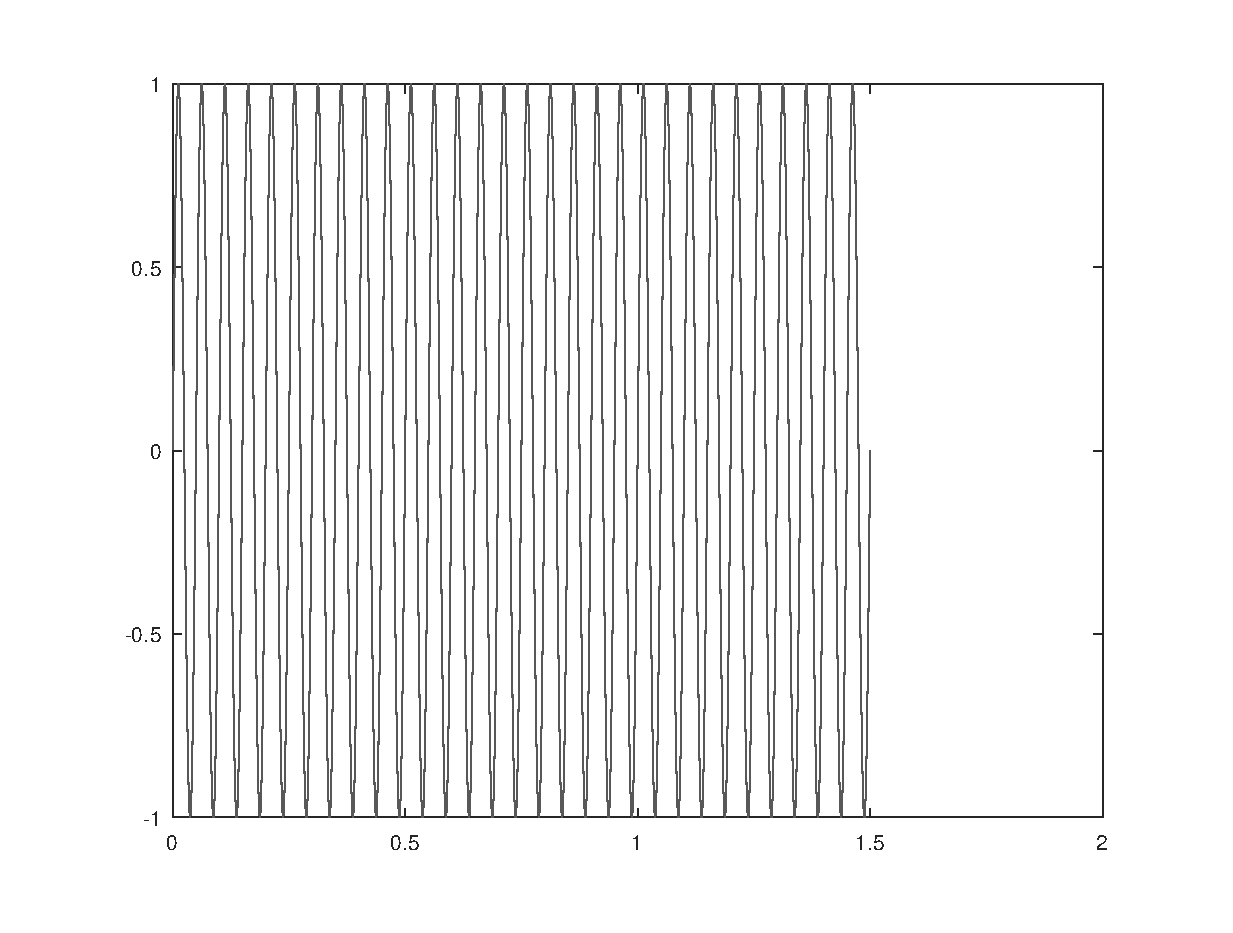
\includegraphics[width=8cm]{figures/modulaciok_workshop_szinusz.eps}
\caption{20 Hz-es szinusz függvény ábrázolása időtartományban}
\label{fig:szinusz}
\end{center}
\end{figure}

A 20 Hz-es jelet könnyen ábrázoltuk, de a hallható tartomány magasabb frekvencián van. Változtassuk a frekvenciát 440 Hz-re (zenei A hang), és játsszuk ki a számítógép hangkártyáján a jelet: \\
\texttt{soundsc(y, Fs); } \\
Itt már több információt kapnánk a jelről, ha frekvenciatartományban, vízesés diagramon ábrázolnánk a jelet. A HA5KFU Octave gyakorlathoz csomagolt \textit{wf(y, Fs)} függvénnyel ezt a rádiózásban megszokott formában rajzolhatjuk ki.

\begin{figure}[H]
\begin{center}
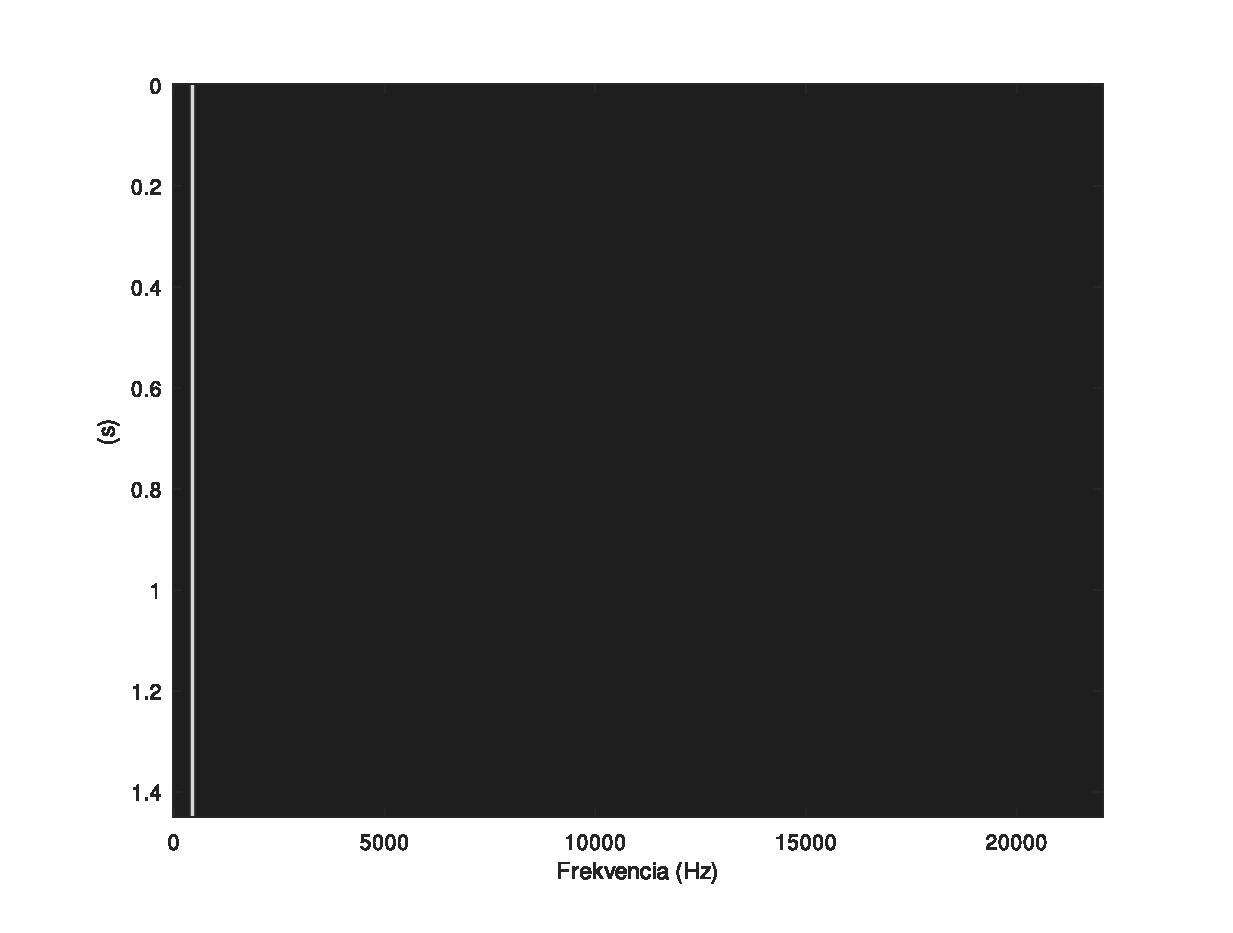
\includegraphics[width=8cm]{figures/modulaciok_workshop_waterfall.eps}
\caption{440 Hz-es szinusz függvény ábrázolása frekvenciatartományban}
\label{fig:waterfall}
\end{center}
\end{figure}

A vízesés diagram 0-tól a mintavételi frekvencia feléig ábrázolja a frekvenciakomponenseket, az ábrán láthatjuk a konstans szinusz jel képét 440 Hz-nél. Próbálkozzunk meg a jel manipulálásával, hallgassuk meg, ábrázoljuk frekvenciatartományban!\\
\lstinline{y = ( 1 - ( 1 / l ) * t ) .* sin( t * f * 2 * pi ); % Fokozatosan halkulo jel } \\
\lstinline{y = sin( t .* ( f * t ) * 2 * pi ); % Valtozo frekvenciaju szinusz } \\
\lstinline{y = sin( t * f * 2 * pi ) + sin( t * 1.5*f * 2 * pi ) ; % Tobb szinusz osszege }
\\
Megpróbálhatunk fehér zajt generálni, vagy hangfilet betölteni is. \\
\lstinline{y = rand( N, 1 ) ; % N elemu zaj}  \\
\lstinline{[y,Fs] = audioread('akkord.wav'); % WAV file beolvasasa}

\clearpage

\subsection{Keverés}

\end{document}
